\documentclass[10pt,twocolumn,letterpaper]{article}
\usepackage[margin=1in]{geometry}
\usepackage[T1]{fontenc}
\usepackage{newtxtext,newtxmath}
\renewcommand{\ttdefault}{lmtt}
\usepackage{graphicx,booktabs,tabularx,array,xcolor,caption,enumitem,longtable,microtype}
\usepackage[round]{natbib}
\usepackage[hidelinks]{hyperref}

\setlength{\columnsep}{0.25in}
\setlist{nosep,leftmargin=1.2em}
\setlist[itemize]{label=$\bullet$}
\captionsetup{font=small,labelfont=bf,skip=4pt}
\renewcommand{\arraystretch}{1.08}
\setcounter{topnumber}{3}\setcounter{totalnumber}{4}
\renewcommand{\topfraction}{0.9}\renewcommand{\dbltopfraction}{0.9}
\renewcommand{\textfraction}{0.08}\renewcommand{\floatpagefraction}{0.8}\renewcommand{\dblfloatpagefraction}{0.8}
\newcolumntype{L}{>{\raggedright\arraybackslash}X}

\definecolor{pendfill}{HTML}{FFF1C2}
\definecolor{pendline}{HTML}{C98500}
% A result that is not in yet. Each one names the run that fills it.
\newcommand{\pend}[1]{\fcolorbox{pendline}{pendfill}{\footnotesize\bfseries PENDING: #1}}
\newcommand{\pendbox}[1]{\par\smallskip\noindent\fcolorbox{pendline}{pendfill}{\parbox{\dimexpr\linewidth-2\fboxsep-2\fboxrule\relax}{\small\textbf{PENDING:} #1}}\par\smallskip}
% A section of the study's results record, results/expanse/README.md.
\newcommand{\sect}[1]{\S#1}

\title{ExeaLM: Long Memory and a Library for Research and Code}
\author{Avneh Bhatia (Exea Labs)\\ \pend{further authors to be decided}}
\date{Draft of 27 November 2026}

\begin{document}
\maketitle

\begin{abstract}
ExeaLM is a language model for research and code.
It is built for inputs longer than the window it reads at once, and for facts its weights cannot hold: it carries a memory from one 512-token window to the next, and it reads entries from a library it ships with.
We trained it against our implementation of the Qwen3.5 layer design at 0.1B, 0.25B and 0.5B parameters, with the same data and tokens, on a 2,000 GPU-hour allocation from the National AI Research Resource Pilot.
On long-context tasks scored as exact match, ExeaLM recalls 12 to 14 percent more text from beyond its window at every size, completes 7 to 10 percent more lines of code that depend on distant definitions, and finds a planted pass key 4 to 50 times as often.
Unlike its lead on short text, which shrinks from 2.8 to 0.6 percent in bits per byte, its recall lead does not shrink with size.
Its memory layer triples retrieval of a pass key from the previous window over the same model with attention in its place.
With its library, a 0.1B ExeaLM scores better on held-out research questions than the released Qwen3.5-9B without one, at about a sixth of the compute per answer.
Trained as long per parameter as the planned 9B, it reaches the Qwen3.5-style model's quality in 25 to 29 percent fewer steps.
A 3B pair finishes after this draft.
\end{abstract}

\begin{figure*}[t]
\centering
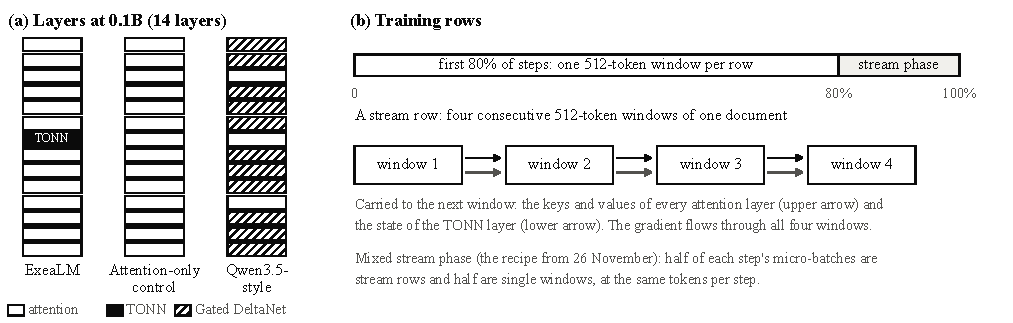
\includegraphics[width=\textwidth]{figs/fig_model.pdf}
\caption{(a) The layers of the three models at 0.1B, with layer 0 at the bottom. ExeaLM is attention everywhere except one TONN layer at the middle layer. The attention-only control puts attention there too, and the Qwen3.5-style model has Gated DeltaNet in three of every four layers. (b) Every model reads one 512-token window per row for its first 80\% of steps. In its last 20\%, ExeaLM reads rows of four consecutive windows of one document, with each window's attention keys and values and the TONN layer's state carried into the next.}
\label{fig:model}
\end{figure*}

%=====================================================================================================
\section{Introduction}

A model that helps with research and code meets two problems that size alone handles poorly.
Its inputs are long: a paper runs 4,000 to 10,000 tokens, and code that spans a repository 8,000 to 32,000, many times the window a small model reads at once.
Its answers also depend on more facts than its weights can hold; plain weights store about 2 bits of knowledge per parameter \citep{allenzhu2024physics}.
A model that is to be the best of its size for research and code, and the cheapest per answer, has to meet both problems with something other than more parameters.

ExeaLM, Exea Labs' language model for research and code, meets them with two parts that do not grow with the model.
For long inputs it reads a document as a \emph{stream}: each 512-token window is read with the attention keys and values of the window before and the state of a memory layer carried in.
That layer, a \emph{TONN layer}, sits at the middle of the network and holds small signal circuits such as short convolutions, running sums and state-space memories.
For facts it reads a \emph{library}: a keyword search picks the best written entry and the best passage of real text for the question, and the model reads them before it answers.
The rest of ExeaLM is a transformer with four published changes to attention.

This report gives the evidence that these parts work, from a scaling study on 2,000 hours of NVIDIA H100 GPUs (GPU-hours) from the National AI Research Resource Pilot.
We compare ExeaLM with a Qwen3.5-style model, our implementation of Qwen3.5's mix of attention and Gated DeltaNet layers \citep{qwen35}, a recurrent design with a matrix memory, and with a plain Llama.
Every model trains at equal size, data and tokens.
We finished 0.1B, 0.25B and 0.5B parameters (B for billion) with 3, 3 and 2 seeds, or independent runs; the 0.1B pair also trained 27 times longer, to the 9B's ratio of tokens to parameters, and a 3B pair is training.
We score models on long-context tasks as exact match, in \emph{bits per byte} on 18 held-out sets (text no model trained on; lower is better), and on benchmarks.

What the study shows:
\begin{itemize}
\item \textbf{ExeaLM remembers more of a long document.} On held-out documents read as a stream, it recalls 14\%, 12\% and 12\% more text last seen beyond its window than the Qwen3.5-style model at 0.1B, 0.25B and 0.5B, completes 10\%, 9\% and 7\% more lines of code that depend on a distant definition, and finds a planted pass key 4 to 50 times as often. Every difference holds target by target ($p \le 0.002$), and the recall lead does not shrink with size (Section~\ref{sec:long}).
\item \textbf{Its memory layer carries exact facts across windows.} With attention in place of the TONN layer, the model finds a pass key one window back 9\% of the time against ExeaLM's 28\% (0.25B, 3 seeds, $p = 3\times10^{-8}$) (Section~\ref{sec:parts}).
\item \textbf{Its library turns a small model into a strong one on research questions.} A 0.1B ExeaLM that reads library entries found by a keyword search cuts its bits per byte on held-out research questions by 64\% (3 seeds), and with the second library, written by DeepSeek-V4-Flash, by 74\%. It then scores better than the released Qwen3.5-9B without a library, at about a sixth of the compute per answer (Sections~\ref{sec:library} and~\ref{sec:cost}).
\item \textbf{It learns more per token.} Trained to 111 tokens per parameter, the Qwen3.5-style model needs 34\% to 41\% more steps to match ExeaLM through step 20,000 (2 seeds), and never reaches its final score (Section~\ref{sec:length}).
\item \textbf{It is ahead on every held-out set.} ExeaLM is ahead of the Qwen3.5-style model on all 54 set-and-seed pairs at 0.1B and 0.25B and all 36 at 0.5B, by 5.3\% to 3.6\% on long documents and 2.8\% to 0.6\% on short windows (Section~\ref{sec:size}).
\item \textbf{The 9B is priced.} At the speed we measured for the 9B on one node, pretraining on 1T tokens takes about 75,000 GPU-hours, \$202,000 to \$299,000 at public prices (Section~\ref{sec:cost}).
\end{itemize}
We also report what did not work, including a retrieval circuit inside the model and a gradient-averaging bug that voided our first multi-GPU runs (Section~\ref{sec:negative}).

What this report does not show yet: results above 0.5B parameters (the 3B pair finishes after this draft and its results are marked pending), library results beyond bits per byte at 0.1B, and retrieval of exact facts from two or more windows back, which no model we trained can do.
On short windows read alone the lead shrinks with size, and on seven zero-shot benchmarks the 0.5B models differ by less than 0.01 in mean accuracy.

%=====================================================================================================
\section{Model and training}
\label{sec:model}

Figure~\ref{fig:model} shows the three layer stacks and the rows ExeaLM reads in training.

\subsection{ExeaLM}

ExeaLM is a decoder-only transformer \citep{vaswani2017attention}.
Each layer mixes information across positions and is followed by a gated feed-forward block \citep{shazeer2020glu}.
Every layer but one is attention with four published changes.
\begin{itemize}
\item An \emph{output gate} multiplies each attention output channel by a sigmoid of the layer's input \citep{qiu2025gated}.
\item \emph{QK-norm} normalizes each head's queries and keys before their dot product \citep{henry2020qknorm}.
\item \emph{Value residual} mixes the first attention layer's values into the values of each later attention layer, with two learned weights \citep{zhou2024value}.
\item \emph{Exclusive self-attention} (XSA) removes from each head's output its component along the token's own value \citep{zhai2026xsa}.
\end{itemize}

The middle layer is a TONN layer: layer 7 of 14 at 0.1B, 8 of 16 at 0.25B, 11 of 22 at 0.5B and 17 of 34 at 3B.
A TONN layer projects its input into slots of 32 channels and runs one small circuit in each slot.
The circuits include short convolutions, delays, products of two inputs, leaky and gated running sums, and softmax pooling over the past.
They also include a selective state space like Mamba's \citep{gu2023mamba} and an oscillating memory like S4D \citep{gu2022s4d}.
Each slot's output is divided by its running average size, measured on past batches, so no slot drowns out the others.
A second projection adds the slots' outputs back to the layer's input, and the two projections cost as much as attention's four.
The circuits are drawn once at the start, with short convolutions four times as likely as most types, and do not change in training.
Section~\ref{sec:layout} gives the tests that put a single TONN layer at the middle layer.

\begin{table*}[t]
\centering\small
\caption{Bits per byte on held-out text at equal data and tokens (lower is better). ``Windows alone'' is the mean of 18 held-out sets, each 512-token window read by itself. ``Long documents'' is the first 4,096 tokens of each long held-out document read as a stream of 8 windows, mean of windows 1 to 7. Pairs counts the set-and-seed pairs on which ExeaLM is ahead of the Qwen3.5-style model on windows alone. Leads are computed before rounding.}
\label{tab:main}
\footnotesize\setlength{\tabcolsep}{4.2pt}
\begin{tabular}{@{}l c ccc c cc c c l@{}}
\toprule
& & \multicolumn{4}{c}{Windows alone} & \multicolumn{3}{c}{Long documents} & & \\
\cmidrule(lr){3-6}\cmidrule(lr){7-9}
Size, tokens per parameter & Seeds & ExeaLM & Qwen3.5-style & Llama & Lead & ExeaLM & Qwen3.5-style & Lead & Pairs & Record \\
\midrule
0.1B, 4 & 3 & \textbf{1.157} & 1.190 & 1.200 & 2.8\% & \textbf{1.096} & 1.157 & 5.3\% & 54 of 54 & \sect{9}, \sect{10} \\
0.25B, 4 & 3 & \textbf{1.014} & 1.026 & 1.041 & 1.1\% & \textbf{0.955} & 0.997 & 4.2\% & 54 of 54 & \sect{13}, \sect{15} \\
0.5B, 4 & 2 & \textbf{0.933} & 0.939 & 0.958 & 0.6\% & \textbf{0.873} & 0.906 & 3.6\% & 36 of 36 & \sect{20} \\
0.1B, 110 (long runs) & 2 & \textbf{0.958} & 0.963 & not trained & 0.6\% & \textbf{0.902} & 0.946 & 4.7\% & 33 of 36 & \sect{24} \\
3B, 4, step 7,500$^{*}$ & 1 & \textbf{0.850} & 0.866 & not trained & 1.9\% & \multicolumn{3}{c}{after training} & & \sect{23} \\
3B, 4, final & 1 & \multicolumn{9}{l}{\pend{3B final, both readings, from the 3B pair due on the evening of 29 November 2026}} \\
\bottomrule
\end{tabular}
\par\smallskip\raggedright\footnotesize $^{*}$In-run check at step 7,500 of 45,688, before the stream phase and the anneal mix. It reads 512 fixed held-out windows alone, a different reading from the 18-set mean of the other rows.
\end{table*}

\subsection{Baselines and the control}

The \emph{Qwen3.5-style model} follows the layer pattern of Qwen3.5 \citep{qwen35}.
Three of every four layers are Gated DeltaNet \citep{yang2025gated}, and the fourth is attention with the output gate and QK-norm.
Gated DeltaNet is a recurrent layer that keeps a matrix memory for each head, decays it at each token and writes a new value under the token's key.
This is our implementation, trained on our data, and not Alibaba's released model.
Its Gated DeltaNet runs in plain PyTorch from 0.1B to 0.5B and on the flash-linear-attention kernel \citep{yang2024fla} at 3B, and the two agree in 32-bit precision (\sect{6}).
The \emph{plain Llama} has attention in every layer, with none of the four changes \citep{touvron2023llama}.
It trains from 0.1B to 0.5B as a reference.
The \emph{attention-only control} is ExeaLM with its TONN layer replaced by an attention layer with the same four changes.
It trains with ExeaLM's full recipe, so it measures what the TONN layer adds.
All models share a 32,768-token tokenizer, tied input and output embeddings, root-mean-square normalization \citep{zhang2019rmsnorm}, rotary positions \citep{su2024roformer} and attention heads 64 channels wide (Appendix~\ref{app:hyper}).

\subsection{Streams and the stream phase}
\label{sec:streams}

A \emph{window} is 512 consecutive tokens.
For the first 80\% of training steps, every model reads one window per row.
In ExeaLM's last 20\%, the \emph{stream phase}, each row holds four consecutive windows of one document, 2,048 tokens in all.
Each window is read with the keys and values of every attention layer from the window before, as in Transformer-XL \citep{dai2019transformerxl}, and with the TONN layer's state.
The gradient flows through all four windows, a form of truncated backpropagation through time \citep{williams1990tbptt}.
A step holds the same tokens in either phase, so a stream-phase step sees a quarter as many documents.
Exact attention reaches one window back, and older text reaches the model only through the TONN layer's state.
The baselines read one window per row for the whole run.
We made the stream phase part of ExeaLM's recipe and did not give it to the baselines.
Any model could train this way, so Section~\ref{sec:parts} separates its effect.

A step adds up several forward and backward passes, called micro-batches.
On 26 November we changed the recipe to a \emph{mixed stream phase}, in which half of each step's micro-batches are stream rows and half are single windows.
The change applies to the runs whose stream phase had not begun, which are the 3B ExeaLM and the second seed of the long 0.1B run.
The finished 0.1B to 0.5B runs and the first long seed keep the original stream phase.
Section~\ref{sec:recipe} gives the reasons.

\subsection{Recipe and data}

Every step trains on 262,144 tokens, with AdamW \citep{loshchilov2019adamw}, weight decay 0.1 and gradient clipping at 1.0, in the 16-bit bfloat16 number format.
The learning rate warms up over the first 5\% of steps, holds, and decays linearly over the last 20\% to a tenth of its peak.
The last 10\% of steps read the \emph{anneal mix}, which reweights the same sources.
It counts worked code and math solutions and Stack Exchange three times their base share.
Research Python, papers, English Wikipedia and question-answer text count twice, math and Japanese Wikipedia one and a half times, and web text half.
All runs read \texttt{slice-30b-r2} of our public pretraining set, 28.5B tokens after removing duplicates and text that overlaps test benchmarks, 7.3B of them research code.
The mix puts research code first, then general code and research papers, with math, web text, Japanese and question-answer text.
The largest run reads 12.0B tokens, so no run reads any text twice.

%=====================================================================================================
\section{Setup}
\label{sec:setup}

\paragraph{Sizes and seeds.}
We train at 0.1B, 0.25B and 0.5B parameters with 3, 3 and 2 seeds, and at 3B with one seed.
A \emph{seed} fixes a run's random choices, which are its starting weights, starting circuits and data order.
At each size every model trains for the same steps on the same tokens: 0.38B, 1.0B, 2.1B and 12.0B tokens.
That is 4.0 tokens per ExeaLM parameter, although the run names say 4.1, the ratio planned for an earlier layout.
ExeaLM and the Qwen3.5-style model have the same number of parameters within 1\%, and the plain Llama has about 6\% fewer.
The long runs train the 0.1B ExeaLM and Qwen3.5-style model for 39,735 steps on 10.4B tokens, with 2 seeds each.
That is about 110 tokens per parameter, close to the 108 of a 9B model trained on one trillion tokens.

\paragraph{Learning rates.}
Each model gets its own peak learning rate at each size from short checks.
The checks try 3e-4, 6e-4 and 1e-3 for 1,000 steps at 0.1B to 0.5B, and 3e-4 and 6e-4 for 500 steps at 3B (Appendix~\ref{app:hyper}).

\paragraph{Held-out text.}
Scores come from 18 held-out sets, one for each source of the training mix.
They range from research Python and worked code solutions to papers, math, web text and Japanese (Appendix~\ref{app:sets}).
From each set, every model reads the same 512 windows of 512 tokens.
Bits per byte is the model's loss on this text in bits, divided by the number of bytes.
Counting per byte lets models with different tokenizers be compared.

\paragraph{Readings.}
We score each finished model in three ways, and follow training with a fourth.
\begin{itemize}
\item \emph{Windows alone}: the mean over the 18 sets with each 512-token window read by itself.
\item \emph{Long documents}: the first 4,096 tokens of every held-out document at least that long, up to 64 per set, read in order as 8 windows. Each window carries in the attention keys and values of the window before, plus the TONN layer's state for ExeaLM and the Gated DeltaNet memory for the Qwen3.5-style model. We report the mean of windows 1 to 7, since window 0 has nothing before it. As a reference, we also read the same windows alone.
\item \emph{16,384-token documents}: the same over 32 windows, for up to 40 documents per set from the 15 sets that have them.
\item \emph{In-run check}: while it trains, each run scores 512 fixed held-out windows, each read alone, every 500 steps. The windows are the same for every model. We label it wherever we quote it.
\end{itemize}

\paragraph{Leads and pairs.}
ExeaLM's \emph{lead} is the Qwen3.5-style model's bits per byte minus ExeaLM's, each averaged over seeds.
A percentage lead divides this difference by the Qwen3.5-style model's score.
A \emph{set-and-seed pair} compares the two models trained with the same seed on one held-out set, so 3 seeds give 54 pairs.

\paragraph{Step multiplier.}
For each in-run check of an ExeaLM run, we find the step at which the paired Qwen3.5-style run first reaches the same score.
The \emph{step multiplier} is that step divided by ExeaLM's step.
The two runs read the same tokens per step and have the same size within 1\%, so it is also a multiplier on training tokens.

\paragraph{The record.}
Each result has a section in the study's results record, \texttt{results/expanse/README.md}, which we cite as \sect{N}.
Appendix~\ref{app:sources} maps every number to its file.

\begin{figure*}[t]
\centering
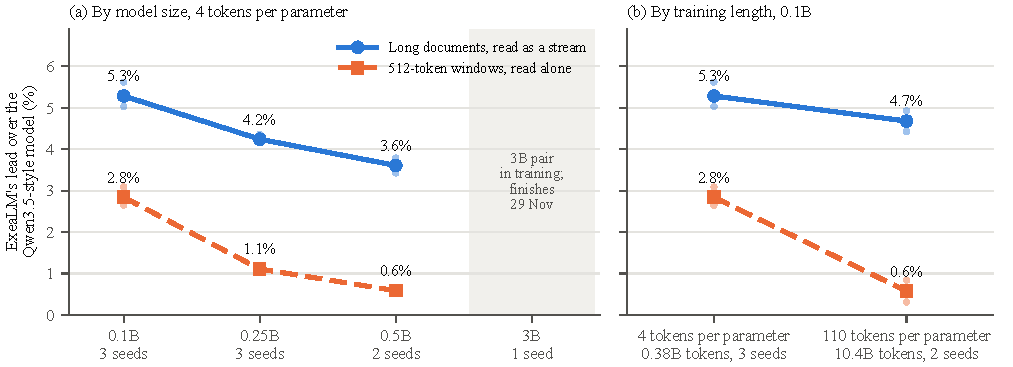
\includegraphics[width=\textwidth]{figs/fig_trends.pdf}
\caption{ExeaLM's lead over the Qwen3.5-style model, as a percentage of the Qwen3.5-style model's bits per byte. Blue is long documents read as a stream (4,096 tokens), and orange is 512-token windows read alone. Large markers are means over seeds, and small dots are single seeds. (a) By model size at 4 tokens per parameter. (b) At 0.1B, by training length. Both leads shrink, and the long-document lead shrinks less.}
\label{fig:trends}
\end{figure*}

%=====================================================================================================
\section{Results across size}
\label{sec:size}

Table~\ref{tab:main} gives the scores at each finished size, with the long runs and the 3B in-run check below them.

\paragraph{Windows alone.}
At 0.1B, ExeaLM scores 1.157 against 1.190 bits per byte for the Qwen3.5-style model (3 seeds).
It is ahead on all 54 set-and-seed pairs, by 0.024 to 0.061.
At 0.25B it scores 1.014 against 1.026 (3 seeds), ahead on all 54 pairs by 0.007 to 0.026.
At 0.5B it scores 0.933 against 0.939 (2 seeds), ahead on all 36 pairs by 0.002 to 0.013.
The two 0.5B seeds of each model agree within 0.0003.
ExeaLM is also ahead of the plain Llama on every pair at every size, by 0.017 to 0.065.
Its lead over the Qwen3.5-style model is largest on the two Japanese sets at every size (Appendix~\ref{app:sets}).

\paragraph{The lead shrinks with size.}
Figure~\ref{fig:trends}a shows the lead on windows alone falling from 0.034 bits per byte (2.8\%) at 0.1B to 0.011 (1.1\%) at 0.25B and 0.0055 (0.6\%) at 0.5B.
The in-run checks show where the 0.5B lead went.
It was 0.011 at step 6,000 of 7,825 and 0.004 at the end, a stretch that is mostly the stream phase (\sect{20}, seed 0).
At 0.25B the in-run lead was 0.020 at step 2,500, before the stream phase, and the final lead on windows alone is 0.011 (\sect{13}).
Section~\ref{sec:recipe} measures what the stream phase costs on windows alone.

\paragraph{Long documents.}
On long documents read as a stream, the lead is larger and shrinks less with size.
It is 0.061 (5.3\%) at 0.1B, 0.042 (4.2\%) at 0.25B and 0.033 (3.6\%) at 0.5B, and ExeaLM is ahead on every set-and-seed pair at each size.

\paragraph{The 3B pair.}
The 3B pair trains for 45,688 steps on 12.0B tokens, one seed of each model.
At step 14,500 its in-run check reads 0.806 for ExeaLM against 0.813.
That lead has narrowed from 0.034 at step 3,000 to 0.016 at step 7,500 and 0.007 at step 14,500 (\sect{23}), about 0.001 every 1,000 steps.
At that rate the two models will be about even on windows alone before the stream phase.
Early leads narrowed in this way at every size in the study; the long-document reading, where the lead held at every finished size, is read on the finished models.
The 3B ExeaLM uses the mixed stream phase, which begins near step 36,550.
\pendbox{3B pair (\texttt{exealm\_3b\_4.1x\_s0}, \texttt{qwen\_3b\_4.1x\_s0}): final windows-alone and long-document scores, set-and-seed pairs, and a 3B point in Figure~\ref{fig:trends}a. Due on the evening of 29 November 2026.}

\paragraph{Benchmarks at 0.5B.}
We score the three 0.5B models (2 seeds each) on seven zero-shot benchmarks, meaning the prompt has no worked examples, with the lm-eval toolkit \citep{gao2024eval}.
Table~\ref{tab:bench} in Appendix~\ref{app:extra} gives each task.
The mean accuracy is 0.429 for ExeaLM, 0.421 for the Qwen3.5-style model and 0.417 for the Llama.
ExeaLM is ahead of the Qwen3.5-style model in both seeds and on 5 of 7 tasks.
Its largest gaps are on SciQ (0.032) and LAMBADA (0.020), which asks for the last word of a passage.
At 2.1B training tokens all three models are near chance on ARC-Challenge (chance 0.25) and WinoGrande (chance 0.5).


\paragraph{Benchmarks with the library at 0.1B.}
We score four 0.1B models (seed 0) closed-book and open-book: ExeaLM and the Qwen3.5-style model, each as pretrained and after RAG post-training (Section~\ref{sec:library}).
Open book places the top passage of each library tier before the question, 384 tokens each, and both models get the same library and search.
Entries that share a 13-token window with any of 14 benchmarks are never given, which excludes 10 of v1's 18,545.
Given the library, the post-trained ExeaLM gains on four of five tasks (ARC-Easy 0.349 to 0.361, ARC-Challenge 0.212 to 0.229; mean without MMLU 0.384 to 0.393).
The post-trained Qwen3.5-style model loses with it (0.372 to 0.364), most on SciQ (0.654 to 0.630).
MMLU stays at chance (0.23) for every model.
This is one seed at 0.1B, and no single gain is beyond two standard errors, so we report it as a lead (\sect{25}).

\pendbox{Benchmarks at 3B, from the finished 3B pair. Open-book benchmarks at 0.5B after RAG post-training on library v2 (running), with the 268 v2 entries that overlap a benchmark taken out of the post-training items before any benchmark is read.}

%=====================================================================================================
\section{Training length}
\label{sec:length}

The long runs train the 0.1B models 27 times longer than the runs at 4 tokens per parameter, to about 110 tokens per parameter.
Figure~\ref{fig:trends}b and Table~\ref{tab:long} follow it.

\paragraph{Final scores.}
ExeaLM scores 0.958 against 0.963 on windows alone and 0.902 against 0.946 on long documents (2 seeds).
It is ahead in both seeds on both readings.
On windows alone it is ahead on 33 of 36 set-and-seed pairs.
The three exceptions are seed 0 on worked code solutions, math code and data-science text, each by 0.0003 or less.
On long documents it is ahead on all 36 pairs.
On windows alone the lead falls from 0.034 at 4 tokens per parameter to 0.0055 at 110, as it falls with size.
On long documents it falls less, from 0.061 to 0.044 (5.3\% to 4.7\%).

\begin{table}[t]
\centering\small
\caption{The long runs at 0.1B (\sect{24}). The lead is the in-run check's Qwen3.5-style score minus ExeaLM's. The multiplier is the Qwen3.5-style run's steps to reach ExeaLM's score, divided by ExeaLM's steps. Seed 0 has the original stream phase, and seed 1 the mixed one. Both stream phases and both learning-rate decays begin at step 31,788.}
\label{tab:long}
\setlength{\tabcolsep}{4pt}
\begin{tabular}{@{}r cc cc@{}}
\toprule
& \multicolumn{2}{c}{In-run lead} & \multicolumn{2}{c}{Step multiplier} \\
\cmidrule(lr){2-3}\cmidrule(lr){4-5}
Step & Seed 0 & Seed 1 & Seed 0 & Seed 1 \\
\midrule
5,000 & 0.015 & 0.016 & 1.18 & 1.21 \\
10,000 & 0.009 & 0.012 & 1.21 & 1.31 \\
15,000 & 0.010 & 0.011 & 1.30 & 1.30 \\
20,000 & 0.008 & 0.011 & 1.34 & 1.41 \\
31,500 & 0.009 & 0.011 & & \\
33,000 & 0.001 & 0.008 & & \\
36,000 & 0.003 & 0.006 & & \\
39,735 (end) & 0.002 & 0.007 & \multicolumn{2}{c}{not reached} \\
\bottomrule
\end{tabular}
\end{table}

\paragraph{Step multiplier.}
Through step 20,000 the multiplier rises in both seeds, from 1.18 and 1.21 at step 5,000 to 1.34 and 1.41.
At step 20,000 the Qwen3.5-style model needs a third or more extra steps to match ExeaLM, while the gap in bits per byte narrows.
After step 20,000 the matching step falls inside the Qwen3.5-style run's own learning-rate decay, where its score drops fast.
The multiplier then compares unlike phases of training, so we stop it at step 20,000.
Neither finished Qwen3.5-style run reaches ExeaLM's final in-run score.
Seed 0 kept the original stream phase, and seed 1 switched to the mixed one at step 28,400 (Section~\ref{sec:recipe}).

\paragraph{The attention-only control at the same length.}
The control trained the same 39,735 steps with the original stream phase, like ExeaLM's seed 0 (\sect{24}; one seed each).
It is ahead of ExeaLM on all three readings: 0.958 against 0.960 on windows alone (17 of 18 sets), 0.898 against 0.902 on long documents read as a stream (all 18 sets, by 0.002 to 0.007), and 0.991 against 0.993 on the same documents read window by window.
Both are far ahead of the Qwen3.5-style model on long documents (0.944).
So on plain text at the 9B's ratio of tokens to parameters, ExeaLM's lead over the Qwen3.5 design comes from its four attention changes and its stream training.
This control measures the TONN layer as a plain text layer: these runs train without the memory circuits (library search, board and weight edits), which are TONN circuits that an attention layer cannot hold.
The 9B keeps its TONN layer for those circuits.
ExeaLM's seed 1, with the mixed stream phase, scores 0.956 and 0.902; the stream recipe moves these numbers by as much as the gap.

\pendbox{A 0.5B three-way run at 20 tokens per parameter, one seed, 38,173 steps and 10.0B tokens each, started 27 November. Its models are ExeaLM with the mixed stream phase, the attention-only control and the Qwen3.5-style model. It tests whether these trends hold at a larger size and whether the TONN layer helps in long training.}

%=====================================================================================================
\section{Long documents}
\label{sec:long}

Long documents test what a model does with the text before its current window.
This section asks where ExeaLM's larger lead on them comes from, and how far it reaches.

\paragraph{Models that never trained on streams.}
The baselines never trained on streams, and they differ in what they gain from the carried state.
At 0.1B the Qwen3.5-style model's matrix memory helps it, from 1.230 with each window read alone to 1.157 streamed, a gain of 0.073 (3 seeds, \sect{10}).
The plain Llama gets worse, from 1.238 alone to 1.584 streamed at 0.1B (3 seeds), and from 0.990 to 1.059 at 0.5B (2 seeds, \sect{20}).
Its attention never saw keys and values from an earlier window in training.

\paragraph{Without the stream phase.}
Part of ExeaLM's long-document lead is its stream phase.
The same ExeaLM trained without a stream phase still leads the Qwen3.5-style model on long documents, 1.132 against 1.157 (2.1\%, 3 seeds).
It is ahead on all 54 set-and-seed pairs, with neither model trained on streams (\sect{10}).
The carried state gains this ExeaLM 0.055 over reading the windows alone, and the study's ExeaLM 0.099.

\begin{figure}[t]
\centering
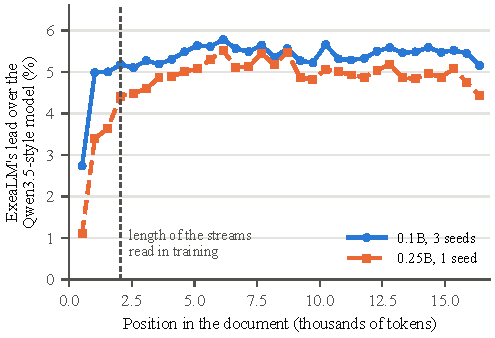
\includegraphics[width=\linewidth]{figs/fig_position.pdf}
\caption{ExeaLM's lead over the Qwen3.5-style model for each 512-token window of held-out documents 16,384 tokens long, as a percentage of the Qwen3.5-style model's bits per byte (\sect{19}). Each point is plotted at the end of its window. The lead is smallest in the first window, which has nothing before it, and stays near 5\% to the end, far past the 2,048 tokens of the training streams.}
\label{fig:position}
\end{figure}

\paragraph{16,384-token documents.}
Figure~\ref{fig:position} follows the lead through documents of 16,384 tokens read as 32 windows, eight times the length of the training streams.
Over windows 1 to 31 ExeaLM scores 1.0726 against 1.1339 at 0.1B (5.4\%, 3 seeds) and 0.9471 against 0.9956 at 0.25B (4.9\%, one seed) (\sect{19}).
Every model keeps improving deeper into the document.
At 0.25B (one seed) the lead is 0.043 in windows 1 to 7 and 0.048 in windows 24 to 31, though it dips in the last few windows.
At 0.1B it stays between 5.0\% and 5.8\% from the second window to the last.

\paragraph{Long-context tasks.}
Bits per byte is a proxy for the tasks a research or code assistant does, which are exact.
We score every finished model on three over the first 4,096 tokens of held-out documents read as a stream (\sect{26}).
\emph{Recall} asks for the last 4 tokens of a 6-token run last seen more than a window back, so neither the window nor the carried keys and values hold it.
\emph{Code next line} asks for a line that uses an identifier last seen more than a window back, the next-line task of RepoBench \citep{liu2023repobench} within one file.
\emph{Pass key} plants a 5-digit number in Wikipedia text and asks for it in the last window, as in RULER \citep{hsieh2024ruler}.
A target counts only if the top token is right at every position, which is what greedy decoding would write.
Table~\ref{tab:longctx} gives the rates.
Against the Qwen3.5-style model ExeaLM is ahead on every task at every size, and every difference holds target by target (McNemar's test, p at most 0.002).
Its recall lead is 14\%, 12\% and 12\% at 0.1B, 0.25B and 0.5B: unlike the lead in bits per byte, it does not shrink with size.
The Qwen3.5-style model also finds the pass key less often with nothing carried (0.30, 0.07 and 0.35 against 0.69, 0.68 and 0.80), so part of the gap is its three-in-four recurrent layers, not only the streams.
No model finds the pass key two or more windows back.

\begin{table}[t]
\centering\small
\setlength{\tabcolsep}{3pt}
\caption{Long-context tasks, exact-match rate read as a stream, mean over seeds (0.1B and 0.5B: 2; 0.25B: 3). The 0.1B pair trained to 111 tokens per parameter. PK: pass key in the same window and one window back.}
\label{tab:longctx}
\begin{tabular}{@{}l cccc@{}}
\toprule
Model & Recall & Code line & PK same & PK back \\
\midrule
ExeaLM, 0.1B & 0.268 & 0.042 & \textbf{0.648} & \textbf{0.078} \\
Qwen3.5-style, 0.1B & 0.235 & 0.038 & 0.047 & 0.000 \\
ExeaLM, 0.25B & 0.241 & 0.035 & \textbf{0.766} & \textbf{0.281} \\
Attention-only, 0.25B & 0.243 & 0.035 & 0.635 & 0.094 \\
Qwen3.5-style, 0.25B & 0.215 & 0.032 & 0.016 & 0.000 \\
ExeaLM, 0.5B & \textbf{0.282} & \textbf{0.045} & \textbf{0.859} & \textbf{0.266} \\
Qwen3.5-style, 0.5B & 0.252 & 0.042 & 0.188 & 0.000 \\
Plain Llama, 0.5B & 0.186 & 0.027 & 0.000 & 0.000 \\
\bottomrule
\end{tabular}
\end{table}

%=====================================================================================================
\section{What each part adds}
\label{sec:parts}

Table~\ref{tab:parts} collects the controls at 0.1B, each with 3 seeds.

\begin{table}[t]
\centering\small
\caption{Controls at 0.1B and 0.25B, 3 seeds each, bits per byte (lower is better) on windows alone and on documents of 4,096 and 16,384 tokens read as a stream. Every ExeaLM variant trains with the same data, steps and learning rate, and the control with the same data, steps and recipe. Dashes mark readings not run.}
\label{tab:parts}
\setlength{\tabcolsep}{3pt}
\begin{tabular}{@{}l ccc@{}}
\toprule
Model & Alone & 4,096 & 16,384 \\
\midrule
ExeaLM (stream phase) & 1.1566 & \textbf{1.0955} & \textbf{1.0726} \\
Attention-only control & 1.1574 & 1.0969 & 1.0737 \\
ExeaLM, no stream phase & \textbf{1.1496} & 1.1321 & -- \\
ExeaLM, mixed, last 20\% & 1.1532 & 1.0969 & -- \\
ExeaLM, mixed, last 40\% & 1.1546 & 1.0956 & -- \\
ExeaLM, weights averaged & 1.2085 & 1.1523 & -- \\
Qwen3.5-style & 1.1904 & 1.1566 & 1.1339 \\
Plain Llama & 1.1995 & 1.584 & -- \\
\midrule
ExeaLM, 0.25B & \textbf{1.0141} & \textbf{0.9545} & -- \\
Attention-only control, 0.25B & 1.0154 & 0.9556 & -- \\
\bottomrule
\end{tabular}
\end{table}

\subsection{The TONN layer}

At 0.1B, ExeaLM scores 1.1566 against 1.1574 for the attention-only control on windows alone.
It is ahead in 2 of 3 seeds and on 40 of 54 set-and-seed pairs.
On 4,096-token documents it scores 1.0955 against 1.0969, and on 16,384-token documents 1.0726 against 1.0737, ahead in all 3 seeds on both (\sect{19}).
The difference is about 0.1\%, and on windows alone it is inside the spread of ExeaLM's seeds (1.1549 to 1.1575).
On exact retrieval across windows the TONN layer matters more (\sect{26}).
With attention in its place, the 0.25B model finds a pass key one window back 0.094 of the time against ExeaLM's 0.281 (3 seeds; 38 trials only ExeaLM gets against 2, p = $3\times10^{-8}$), and in the last window of a stream 0.635 against 0.766 (p = $6\times10^{-4}$).
Read window by window with nothing carried, the two are close (0.609 against 0.677, p = 0.10): what the layer adds is in the state it carries.
On recall and code next line the two are even.
The control leads the Qwen3.5-style model by nearly as much as ExeaLM does.
The lead over the Qwen3.5-style model therefore comes from ExeaLM's attention layers, with their four changes.
On long documents the stream phase adds to it, and on windows alone it takes some away (Section~\ref{sec:recipe}).
At 0.25B, ExeaLM is ahead of the attention-only control on every reading, 3 seeds each: 1.0141 against 1.0154 on windows alone (all 3 seeds, 48 of 54 set-and-seed pairs) and 0.9545 against 0.9556 on 4,096-token documents (2 of 3 seeds; \sect{19}).
The control has attention where the Qwen3.5-style model has Gated DeltaNet, so these runs do not separate the four changes from that swap.
Section~\ref{sec:layout} gives a short test that does.

In longer training the control is ahead of ExeaLM.
Trained to 110 tokens per parameter, it beats ExeaLM on all three readings, by 0.4\% on long documents (Section~\ref{sec:length}, one seed each).
\pendbox{The 0.5B three-way run at 20 tokens per parameter is in the box of Section~\ref{sec:length}.}

\subsection{Layouts and attention changes, at 49 million tokens}
\label{sec:layout}

Before the main runs we tested layouts at 0.1B for 3,000 steps of 16,384 tokens, 49 million tokens in all (\sect{3} to \sect{5}, Table~\ref{tab:layout} in Appendix~\ref{app:extra}).
Every model had one learning rate and no stream phase.
ExeaLM's first plan put a TONN layer in every fourth layer.
A Llama with the four attention changes beat it on all 18 sets, 1.349 against 1.376 (3 seeds each).
The layout tests traced the gap to where the TONN layers sat.
One TONN layer at layer 0 scored 1.3867, 0.038 behind one at the middle layer (one seed against three), and each TONN layer beyond one cost more.
One TONN layer at the middle layer scored 1.3484 against the Llama's 1.3493 (3 seeds each).
It was ahead on every seed, by 0.0006 to 0.0013, and on 14 of 18 sets.
We adopted that layout on 26 November.

The same tests compared the non-attention layers.
With a TONN layer in every fourth layer, ExeaLM beat the Qwen3.5-style model with and without value residual and XSA.
It scored 1.401 against 1.420 without them (3 seeds each) and 1.376 against 1.403 with them (1 seed for the Qwen3.5-style model).
The two designs also differ in their share of attention layers, three of four against one of four, so this does not isolate the TONN layer.
Value residual and XSA together gave ExeaLM 0.026 (1.401 to 1.376).
The Qwen3.5-style model with value residual and XSA has all four changes, as does the Llama with them.
These two differ only in Gated DeltaNet against attention in 11 of 14 layers, and they score 1.403 against 1.349 (one seed against three).
At this short length, attention in place of Gated DeltaNet accounts for more of the lead than the two changes do.

\subsection{The stream phase and the mixed recipe}
\label{sec:recipe}

At 0.1B the stream phase costs 0.007 on windows alone, 1.1566 against 1.1496 without it (3 seeds each).
It gains 0.037 on 4,096-token documents, 1.0955 against 1.1321.
Each stream-phase step reads a quarter as many documents, and three of every four windows have the window before in memory.
We tested three ways to keep the gain at less cost (Table~\ref{tab:parts}, and Figure~\ref{fig:recipes} in Appendix~\ref{app:extra} with every seed).
The mixed stream phase over the last 20\% scores 1.1532 on windows alone and 1.0969 on long documents (3 seeds).
It gives back 0.0034 of the 0.0070 the stream phase costs, and gives up 0.0014 of its 0.037 gain.
The same mix over the last 40\% scores 1.1546 and 1.0956.
Averaging the weights of the streamed and unstreamed runs, which differ only in their last 20\%, is worse than either run (1.2085 and 1.1523).
Weight averaging helps when two runs lie in one basin of the loss \citep{frankle2020linear,wortsman2022soups}, and this result suggests these two do not.

The long runs tried each stream phase on one seed (Table~\ref{tab:long}).
With the original stream phase, seed 0's in-run lead fell from 0.009 at step 31,500 to 0.001 at step 33,000 and ended at 0.002.
With the mixed stream phase, seed 1 kept 0.006 to 0.008 through the decay.
On windows alone seed 1 ends 0.008 ahead and seed 0 0.003 ahead.
Seed 1 also entered its stream phase with a larger lead, 0.011 against 0.009.
With one seed per recipe, we cannot separate the recipe from the seed.
The mixed stream phase is now the recipe for runs whose stream phase had not started.

%=====================================================================================================
\section{A searched library}
\label{sec:library}

A small model cannot hold many facts in its weights.
\citet{allenzhu2024physics} measure about 2 bits of knowledge per parameter.
ExeaLM is meant to read facts from a library instead.
We test the simplest form, retrieval-augmented generation (RAG), where a search places a library entry before the question in the model's context \citep{lewis2020rag,ram2023incontext}.

\subsection{Library v1}

Library v1 holds 18,545 entries, 13,548 on research topics and 4,997 on code, 7.9 million tokens in all.
Qwen3-30B-A3B-Instruct-2507 \citep{yang2025qwen3} wrote them from excerpts of source text.
Each entry comes with questions and answers, and with tasks that need the entry adapted.
A hash of each topic puts it on the training side or the held-out side.
The held-out side has 6,253 questions and 6,604 tasks, and we score bits per byte on the answers only.

\paragraph{Search and post-training.}
BM25 \citep{robertson2009bm25}, a standard keyword search, ranks all entries against each item's question, or its instruction and context, over token ids.
The top entry goes before the item.
It is the item's own entry for 86.2\% of questions (93.2\% in the top five) and 72.9\% of tasks (\sect{8}).
We post-train the three finished 0.1B models of ExeaLM and of the Qwen3.5-style model for 600 steps of 65,536 tokens (\sect{7}, \sect{11}).
Half of each step is training-side library items and half is pretraining text.
Half of the library items have the BM25-picked entry before them, as at test time.

\begin{table}[t]
\centering\small
\caption{Bits per byte on the answers to 6,253 held-out research questions (lower is better). ``Library'' places the entry BM25 picks before the question, and ``own entry'' the entry the question was written from (\sect{11}, \sect{18}).}
\label{tab:library}
\setlength{\tabcolsep}{3pt}
\begin{tabularx}{\linewidth}{@{}L c c c c@{}}
\toprule
Model & Seeds & No library & Library & Own entry \\
\midrule
ExeaLM 0.1B & 3 & 1.645 & \textbf{0.590} & 0.405 \\
Qwen3.5-style 0.1B & 3 & 1.633 & 0.704 & 0.529 \\
Qwen3.5-9B-Base (released) & 1 & 1.031 & 0.313 & 0.169 \\
\bottomrule
\end{tabularx}
\end{table}

\paragraph{Results.}
Table~\ref{tab:library} gives the held-out questions.
With the library, ExeaLM's bits per byte fall from 1.645 to 0.590, by 64\% (3 seeds, 0.588 to 0.592).
They fall by 21\% on text tasks and 19\% on code tasks.
Without the library the Qwen3.5-style model is 0.013 ahead on questions, and ExeaLM is 0.017 ahead on text tasks and 0.025 on code tasks.
With the same library and search, ExeaLM is ahead on every seed, by 0.110 to 0.116 on questions and 0.047 to 0.050 on tasks.
Training with searched entries in context gained ExeaLM 0.097 on questions over the same post-training without them (seed 2).

\paragraph{A larger model.}
We also scored the released Qwen3.5-9B-Base \citep{qwen35} on the same items, served with vLLM \citep{kwon2023vllm} (\sect{18}).
These scores count bits over the bytes each model predicts, so tokenizers do not matter.
Without a library it scores 1.031 on the questions, against 0.590 for the 0.1B ExeaLM with its library.
That compares a system with a model.
Given the same library and search, Qwen3.5-9B-Base scores 0.313, far ahead of our 0.1B model.
On the 18 held-out sets without a library, it scores 0.674 against 1.011 for the 0.25B ExeaLM (seed 0).

\paragraph{Limits.}
The model that wrote the entries also wrote the questions, and such questions may suit retrieval better than questions from other writers.
The test scores bits per byte on reference answers and not answer accuracy.
It covers only 0.1B models.

\subsection{Library v2}

Library v2 adds a human tier of real text that no ExeaLM model trained on.
It holds the 90\% of each training source outside the study's slice, plus all of English and Japanese Wikipedia, KAKEN research-grant summaries and Stack Exchange.
That is 25.0B tokens in 36.8 million passages, 44\% research, 28\% Wikipedia, 21\% code, 4\% question-answer text and 2\% math.
It was checked against every held-out set and 14 benchmarks.
A written tier by DeepSeek-V4-Flash, on 150,000 research and 50,000 code topics, is being written.
Searching both tiers in one ranking lets the human passages crowd out the written entries.
For v1's held-out questions, the share with the answer in the top passage falls from 0.74 to 0.44.
Searching the two tiers apart keeps 0.72 for the written tier, and the model reads the top passage of each tier.
On one H100, a pruned GPU index that keeps each token's 100,000 best passages, merged into one table, answers a query over all the passages in 2.0 ms (median).
Its top passage matches the full index's for 86\% of queries (Table~\ref{tab:search} in Appendix~\ref{app:extra}).

\pendbox{Library v2 test: RAG post-training on v2 for ExeaLM and the Qwen3.5-style model with the same recipe, streams included for both, at 0.5B and on a mid-run 3B checkpoint. Fills 0.5B and 3B rows of a table like Table~\ref{tab:library}, and adds held-out documents and questions from which no entry was written.}

%=====================================================================================================
\section{What a result costs}
\label{sec:cost}

A model that is to win on price has to win per unit of compute, not only per parameter.
Four measurements from the study bear on that.

\paragraph{Training steps to a given quality.}
At 0.1B trained to 111 tokens per parameter, the Qwen3.5-style model needs 1.34 and 1.41 times ExeaLM's steps to reach ExeaLM's in-run score at step 20,000 (2 seeds, \sect{24}).
A step is the same tokens for both, and the two have the same parameters within 1\%.
ExeaLM therefore reaches that quality with 25\% to 29\% fewer training tokens and about as much less compute.
After step 20,000 the matching step falls inside the Qwen3.5-style run's learning-rate decay, so we stop the comparison there; the finished Qwen3.5-style runs never reach ExeaLM's final score.

\paragraph{Long-context tasks per parameter.}
At 0.25B ExeaLM finds a pass key in the window it is reading 0.766 of the time, against 0.188 for the Qwen3.5-style model at 0.5B, twice its size, and 0.281 against 0 one window back (both at 4.1 tokens per parameter, \sect{26}).
On recall the larger Qwen3.5-style model is slightly ahead (0.252 against 0.241), and on code next line more so (0.042 against 0.035).
Half the parameters buys most of the recall and four times the retrieval.

\paragraph{An answer with the library.}
On 6,253 held-out research questions, the 0.1B ExeaLM with its library scores 0.590 bits per byte on the answers, and the released Qwen3.5-9B-Base with no library 1.031 (\sect{18}).
A forward pass costs about twice the parameters in operations per token read.
The 0.1B model reads the entry (426 tokens on average) and the question and answer (30), about $2 \times 95\textrm{M} \times 457 \approx 8.7\times10^{10}$ operations; Qwen3.5-9B reads only the question and answer, about $2 \times 9\textrm{B} \times 31 \approx 5.6\times10^{11}$.
The small model with its library is ahead at about a sixth of the compute per answer, plus a keyword search that takes 0.4 ms on a CPU for this library.
This is a system against a model on questions about topics the library covers, and the questions were written by the model that wrote the entries.
Given the same library, Qwen3.5-9B scores 0.313.

\paragraph{The 9B.}
We timed the 9B ExeaLM's full training step on one node of four H100s (\sect{16}).
At that speed, pretraining on 1T tokens takes about 75,000 GPU-hours, \$202,000 to \$299,000 at public on-demand prices of \$2.69 to \$3.99 per GPU-hour.
Qwen3 was pretrained on about 36T tokens \citep{yang2025qwen3}; a 9B run that long at our measured speed would need about 36 times as much.
We do not claim the 9B will match such models token for token.
The bet is that a model which learns more per token, remembers more of a long input and reads a library closes much of that gap on research and code for a small share of the cost; the 3B pair and a scaling fit are the next tests of it.

%=====================================================================================================
\section{What did not work}
\label{sec:negative}

\paragraph{ExeaLM's own retrieval circuit.}
Before using a keyword search, we grafted a retrieval circuit into the trained 0.1B ExeaLM's TONN layer and post-trained it to search the library (\sect{7}).
It returned a chunk of the right entry first for 0.06\% of held-out questions and 7.8\% of tasks (one seed).
Attaching the library moved the question score from 1.6741 to 1.6742.
The entries reached the model only when a search outside it placed them in its context.
Given BM25 candidates in place of its own search (\sect{27}), the circuit's top candidate held the right entry for 89\% of questions, yet the score with the library stayed at 1.725, the same as without it (600 steps, one seed).
Its one attention read, in one slot of one layer, did not learn to use what it found; the same entries pasted into the context brought the score to 0.604.

\paragraph{Agents sharing a board.}
Three 0.1B ExeaLM agents shared a message board, grafted into their TONN layer, while each read one of three consecutive windows (\sect{14}).
After 600 steps of post-training they scored 1.181 on windows 1 and 2 of 1,536-token documents (one seed).
One 0.1B model reading the same windows as a stream scored 1.096.
The board gained 0.0035 over the same agents with the board cut.

\paragraph{Teacher text in pretraining.}
We pretrained the 0.1B ExeaLM with 30\% of its tokens written by Qwen3.5-9B-Base, which continued 200,000 openings of 128 tokens from the training mix (\sect{22}).
It scored 1.1592 against 1.1549 for the same seed trained normally on windows alone, and 1.0986 against 1.0939 on long documents (one seed).

\paragraph{Averaging weights.}
Averaging the weights of a streamed and an unstreamed run was worse than either run on both readings (Section~\ref{sec:recipe}, \sect{21}).

\paragraph{A multi-GPU bug.}
In our training script, the gradient-accumulation loop's variable was overwritten on the loop's first line (\sect{17}).
On more than one GPU with more than two accumulation steps, every backward pass then ran without averaging gradients across GPUs.
Each GPU trained on its own share of each batch, and the in-run check reset the drifting copies to the first GPU's weights.
The 0.5B baselines scored worse than their 0.25B versions, 1.053 and 1.078 against 1.026 and 1.041.
The bug voided the first 0.5B runs, the 0.5B and 3B learning-rate checks and the 3B pair's first 1,100 steps, about 190 GPU-hours.
A test now runs two processes and fails on the old code, and every void run was restarted.
Runs on one GPU were not affected, which covers every 0.1B, 0.25B, long-run and library result.
A smaller bug, fixed in the first job, made the in-run check score streamed runs on a different sample of windows (\sect{1}).
Every finished score we report comes from the separate evaluation scripts.

%=====================================================================================================
\section{Related work}
\label{sec:related}

REALM trained a retriever with a language model in pretraining \citep{guu2020realm}, and RAG paired a dense retriever with a generator \citep{lewis2020rag}.
RETRO retrieved from a database of trillions of tokens \citep{borgeaud2022retro}, and Atlas applied retrieval to few-shot learning \citep{izacard2023atlas}.
In-context retrieval places retrieved documents, found by BM25 among others, before the input of an unchanged model \citep{ram2023incontext}.
Our library test uses that placement and compares how two architectures use the same entries.

Scaling laws relate loss to parameters and tokens \citep{kaplan2020scaling}, and \citet{hoffmann2022chinchilla} found that about 20 tokens per parameter gives the lowest loss for a fixed compute budget.
Our main runs train at 4 tokens per parameter, the long runs at 110, and the pending 0.5B runs at 20.

Transformer-XL caches the previous segment's keys and values \citep{dai2019transformerxl}.
The Compressive Transformer, the Recurrent Memory Transformer and Block-Recurrent Transformers carry a memory or a recurrent state between segments \citep{rae2020compressive,bulatov2022rmt,hutchins2022block}.
ExeaLM's stream phase combines a Transformer-XL cache with the state of one TONN layer, trained only in the last 20\% of steps.

Selective state spaces \citep{gu2023mamba}, diagonal state spaces \citep{gu2022s4d} and Gated DeltaNet \citep{yang2025gated} replace attention with recurrences.
Jamba, Griffin and Qwen3.5 mix such layers with attention \citep{lieber2024jamba,de2024griffin,qwen35}, and our baseline follows Qwen3.5's three-to-one pattern.
Gated attention \citep{qiu2025gated}, QK-norm \citep{henry2020qknorm}, value residual \citep{zhou2024value} and XSA \citep{zhai2026xsa} each change attention alone.
The attention-only control shows that ExeaLM's attention layers with these changes, and its stream phase, account for nearly all of its lead.

Memory layers add large key-value tables that a model reads sparsely \citep{berges2025memory}.
In their abstract, models with memory layers beat dense models with twice the compute, most of all on factual tasks.
We have not tested them.
What this paper adds is a comparison of these parts at three sizes and two training lengths, with controls at 0.1B for the TONN layer and the stream phase.

%=====================================================================================================
\section{Limitations}
\label{sec:limits}

Our models are small.
The largest finished models have 0.5B parameters, and the 3B pair is still training.
The lead on windows alone shrinks with size and with training length, to 0.6\% at 0.5B and to 0.6\% at 0.1B after long training.
We have not fit a trend, and three sizes cannot show whether it reaches zero.
Only ExeaLM trains on streams, and the controls that measure this are at 0.1B.
The Qwen3.5-style model is our implementation of a published layer pattern, trained on our data with our recipe.
Below 3B its Gated DeltaNet runs in plain PyTorch, so we compare models at equal tokens and not at equal time.
In a speed test at 0.5B and 3B, the three designs ran within 16\% of each other per parameter, and the stream phase costs more per token (Appendix~\ref{app:compute}).
Each learning rate comes from short checks of two or three values.
We have 3 seeds at 0.1B and 0.25B, 2 at 0.5B and for the long runs, and 1 at 3B and for several controls.
Bits per byte is not task accuracy, and the 0.5B benchmarks are near chance on two tasks.
The library test uses 0.1B models, questions written by the model that wrote the entries, and bits per byte.
The TONN layer adds about 0.1\% at 0.1B, and trained to 110 tokens per parameter the attention-only control is ahead of ExeaLM on every reading, by 0.4\% on long documents (one seed each).
This paper does not show that the TONN layer is needed.

\section*{Use of generative AI}
Claude Opus 5.5 wrote the first draft of this paper and its figure script from the study's result files and notes.
It also mapped each number to its source in Appendix~\ref{app:sources}.
\pendbox{Authors to check every number and confirm this statement.}

\section*{Impact statement}
\pendbox{Impact statement for the ICML submission, to be written by the authors.}

\section*{Acknowledgments}
This work used an allocation of 2,000 GPU-hours on the San Diego Supercomputer Center's Expanse cluster from the National AI Research Resource Pilot (project \texttt{fli100}).
\pendbox{Full acknowledgments, to be removed for anonymous review.}

\bibliographystyle{plainnat}
\bibliography{refs}

%=====================================================================================================
\clearpage
\onecolumn
\appendix

\section{Where each number comes from}
\label{app:sources}

``\sect{N}'' is section N of \texttt{results/expanse/README.md}.
Files are in \texttt{results/expanse/} unless a path is given.
A percentage lead is the Qwen3.5-style score minus ExeaLM's, divided by the Qwen3.5-style score, computed from unrounded means.
\texttt{paper/make\_figs.py} draws every figure and the table in Appendix~\ref{app:sets} from the JSON files named, and prints the checked numbers.
Counts of set-and-seed pairs, per-pair ranges and the 16,384-token range by window come from its output.

\small\sloppy
\begin{longtable}{@{}>{\raggedright\arraybackslash}p{0.56\linewidth} >{\raggedright\arraybackslash}p{0.40\linewidth}@{}}
\toprule
Number & Source \\
\midrule
\endhead
\bottomrule
\endfoot
0.1B windows alone 1.157, 1.190, 1.200; 54 of 54 pairs, 0.024 to 0.061; Llama 0.033 to 0.065 & \sect{9}, \texttt{text\_100m.json} \\
0.1B long documents 1.096, 1.157; no stream phase 1.132; Qwen3.5-style alone 1.230, gain 0.073; Llama 1.238 and 1.584; gains 0.055 and 0.099 & \sect{10}, \texttt{stream8\_100m.json} \\
0.25B windows alone 1.014, 1.026, 1.041; 0.007 to 0.026 & \sect{13}, \texttt{text\_250m.json} \\
0.25B in-run lead 0.020 at step 2,500 & \sect{13} (the run's training log is not in the repository) \\
0.25B long documents 0.955, 0.997 & \sect{15}, \texttt{stream8\_250m.json} \\
0.5B, 2 seeds: 0.933, 0.939, 0.958; 0.873, 0.906; Llama 0.990 and 1.059; 36 of 36; 0.002 to 0.013; seeds within 0.0003; Llama behind by 0.017 to 0.039 & \sect{20}, \texttt{text\_500m\_all.json}, \texttt{stream8\_500m\_all.json} \\
0.5B in-run lead 0.011 at step 6,000, 0.004 at the end & \sect{20} \\
Leads 2.8\%, 1.1\%, 0.6\%; 5.3\%, 4.2\%, 3.6\%; 0.034, 0.011, 0.0055; 0.061, 0.042, 0.033 & computed from the files above by \texttt{make\_figs.py} \\
Largest per-set leads on the Japanese sets & \texttt{make\_figs.py}, Appendix~\ref{app:sets} \\
Benchmarks at 0.5B, 2 seeds (Table~\ref{tab:bench}) & \sect{20}, \texttt{bench\_<model>\_500m\_4.1x\_s0.json} and \texttt{\_s1.json} \\
3B in-run check 0.850, 0.866 at step 7,500; 0.034 at step 3,000; stream phase near step 36,550 & \sect{23}, \texttt{docs/decisions.md} (26 November, 7 p.m.) \\
Long runs: 0.958, 0.963; 0.902, 0.946; 4.7\%; 33 of 36 and 36 of 36 pairs; exceptions of 0.0003 or less & \sect{24}, \texttt{text\_111x.json}, \texttt{stream8\_111x.json} \\
Long runs, in-run leads and step multipliers (Table~\ref{tab:long}); switch at step 28,400; decay from step 31,788 & \sect{24}, \texttt{docs/decisions.md} (26 November, 7 p.m.) \\
Long runs: 39,735 steps, 10.4B tokens, 109.6 and 108.9 tokens per parameter; 9B at about 108 & \texttt{docs/budget.md} (``The runs''), \texttt{docs/funding\_report/report.tex} \\
16,384-token documents: 1.0726, 1.1339, 0.9471, 0.9956; 5.4\%, 4.9\%; 0.043 to 0.048; 15 of 18 sets; 5.0\% to 5.8\% & \sect{19}, \texttt{stream32\_100m.json} \\
Attention-only control 1.1574, 1.0969, 1.0737; 2 of 3 seeds; 40 of 54 pairs (\sect{19} gives 1.0968; the file's seeds average to 1.0969) & \sect{19}, \texttt{text\_100m\_strong.json}, \texttt{stream8\_100m\_strong.json}, \texttt{stream32\_100m.json} \\
Control in the long run: 1.0316, 1.0348 at step 4,000 & \sect{19} \\
Control in the long run, finished: 0.958, 0.960 (17 of 18 sets); 0.898, 0.902 (18 of 18); 0.991, 0.993 & \sect{24}, \texttt{text\_strong\_111x.json}, \texttt{stream8\_strong\_111x.json} \\
No stream phase 1.1496, 1.1321; mixed 1.1532, 1.0969; mixed 40\% 1.1546, 1.0956; averaged 1.2085, 1.1523; 0.0034 of 0.0070; 0.0014 of 0.037 & \sect{21}, \texttt{text\_100m.json}, \texttt{stream8\_100m.json}, \texttt{text\_mix20distill.json}, \texttt{stream8\_mix20distill.json}, \texttt{text\_mix100m.json}, \texttt{stream8\_mix100m.json}, \texttt{text\_merge100m.json}, \texttt{stream8\_merge100m.json} \\
49M-token tests (Table~\ref{tab:layout}); 0.038 at layer 0; 0.0006 to 0.0013; 14 of 18 sets; 0.026; 1.403 against 1.349 & \sect{3}, \sect{4}, \sect{5}, \texttt{ablation\_100m.json}, \texttt{layout\_100m.json}, \texttt{layout2\_100m.json} \\
Library v1: 18,545 entries, 13,548 and 4,997, 7.9M tokens; 6,253 and 6,604 held-out items & \sect{7} \\
BM25 own entry first 86.2\% (93.2\% in five), 72.9\% of tasks & \sect{8}, \texttt{library\_bm25\_100m.jsonl} \\
RAG post-training: 1.645, 0.590, 0.405; 1.633, 0.704, 0.529; 64\%, 21\%, 19\%; 0.110 to 0.116; 0.047 to 0.050; without the library 0.013, 0.017, 0.025 & \sect{11}, \texttt{library\_rag\_100m\_s0.jsonl} to \texttt{\_s2.jsonl} \\
Gain of 0.097 over post-training without entries (seed 2) & \sect{11}, \texttt{library\_bm25\_100m.jsonl}, \texttt{library\_rag\_100m\_s2.jsonl} \\
Post-training of 600 steps of 65,536 tokens & \sect{7}, \sect{11} \\
Qwen3.5-9B-Base: 1.031, 0.313, 0.169; 0.674 against 1.011 & \sect{18}, \texttt{external\_qwen35\_9b\_base.json} \\
About 2 bits of knowledge per parameter & \citet{allenzhu2024physics}, as cited in \texttt{docs/library.md} \\
Library v2: 25.0B tokens, 36.8M passages, tier shares, 150,000 and 50,000 topics; 0.74, 0.44, 0.72; search times (Table~\ref{tab:search}) & \texttt{docs/library.md} \\
Retrieval circuit 0.06\% and 7.8\% (\texttt{search\_first}); 1.6741, 1.6742 & \sect{7} (which rounds 0.06\% to 0.1\%), \texttt{library\_100m.jsonl} \\
Board 1.181, 1.096, 0.0035 & \sect{14}, \texttt{board\_100m.json} \\
Teacher text 1.1592, 1.1549; 1.0986, 1.0939 & \sect{22}, \texttt{text\_mix20distill.json}, \texttt{stream8\_mix20distill.json} \\
Multi-GPU bug: 1.053, 1.078; 1,100 steps; about 190 GPU-hours & \sect{17}, \texttt{docs/decisions.md} (26 November, 8:30 a.m.) \\
Data: 28.5B tokens, 7.3B research code & \texttt{docs/budget.md} (``The data'') \\
Anneal weights & \texttt{experiments/recipe/}\allowbreak\texttt{exealm\_recipe\_v2.json} \\
Learning-rate checks and picks & \sect{17}, \texttt{experiments/expanse/plan.py}, \texttt{experiments/expanse/lr\_choice.json} \\
Open-book rules: 13-token window, 14 benchmarks, 10 entries & \texttt{docs/decisions.md} (26 November, midnight) \\
0.5B run at 20 tokens per parameter: 38,173 steps, 10.0B tokens & \texttt{docs/decisions.md} (27 November, 1:45 a.m.) \\
Speeds of the study's models (Table~\ref{tab:speed}); within 16\% & \texttt{throughput\_speed\_0.5B\_512\_c0.json}, \texttt{\_c1.json}, \texttt{throughput\_speed\_3B\_512\_c0.json}, \texttt{\_c1.json} (not yet written up in the record) \\
Other speeds and compute (Appendix~\ref{app:compute}) & \sect{1}, \sect{2}, \sect{16}, \texttt{throughput\_h100.json}, \texttt{scaling\_500m.json}, \texttt{nine\_b.json}, \texttt{docs/decisions.md} \\
\end{longtable}
\normalsize

\section{Hyperparameters}
\label{app:hyper}

Table~\ref{tab:hyper} gives each size.
All models use AdamW with $\beta_1 = 0.9$, $\beta_2 = 0.95$ and $\epsilon = 10^{-8}$, weight decay 0.1 on weight matrices other than the embeddings, and gradient clipping at 1.0.
They train in bfloat16 (bf16) on steps of 262,144 tokens.
The learning rate warms up linearly over the first 5\% of steps (at most 2,000), holds, and decays linearly over the last 20\% to 10\% of its peak.
The anneal mix starts at 90\% of steps, and ExeaLM's stream phase at 80\%.
Every model has tied embeddings, RMS normalization before each sublayer, a gated feed-forward block 8/3 the width, rotary positions and attention heads 64 channels wide (\texttt{docs/budget.md}, \texttt{exealm/config.py}, \texttt{exealm/train/pretrain.py}).
ExeaLM's TONN layer has one circuit per 32 channels of width.
The 0.1B and 0.25B runs and the long runs train on one H100, and the 0.5B and 3B runs on four.
The baselines train with \texttt{torch.compile} on one GPU, and ExeaLM trains without it.

\begin{table}[h]
\centering\small
\caption{Model sizes and training per size (\texttt{exealm/config.py}, \texttt{experiments/expanse/*.json}, \texttt{docs/budget.md}, \texttt{experiments/expanse/lr\_choice.json}). Parameters are in millions.}
\label{tab:hyper}
\begin{tabular}{@{}l r r r r r@{}}
\toprule
& 0.1B & 0.25B & 0.5B & 3B & 0.1B long runs \\
\midrule
Width & 640 & 1,024 & 1,280 & 2,560 & 640 \\
Layers & 14 & 16 & 22 & 34 & 14 \\
Attention heads & 10 & 16 & 20 & 40 & 10 \\
Feed-forward width & 1,704 & 2,728 & 3,408 & 6,824 & 1,704 \\
ExeaLM's TONN layer (index) & 7 & 8 & 11 & 17 & 7 \\
TONN circuits & 20 & 32 & 40 & 80 & 20 \\
Qwen3.5-style attention layers & 3 of 14 & 4 of 16 & 5 of 22 & 8 of 34 & 3 of 14 \\
\midrule
ExeaLM parameters & 95.1 & 250.5 & 508.5 & 2,973.5 & 95.1 \\
Qwen3.5-style parameters & 95.7 & 252.1 & 511.3 & 2,986.2 & 95.7 \\
Plain Llama parameters & 89.7 & 234.8 & 474.1 & & \\
Attention-only control parameters & 95.5 & & & & 95.5 \\
\midrule
Steps & 1,468 & 3,869 & 7,825 & 45,688 & 39,735 \\
Tokens & 0.38B & 1.0B & 2.1B & 12.0B & 10.4B \\
Warm-up steps & 73 & 193 & 391 & 2,000 & 1,986 \\
Seeds & 3 & 3 & 2 & 1 & 2 \\
GPUs per run & 1 & 1 & 4 & 4 & 1 \\
\midrule
Peak learning rate, ExeaLM & 1e-3 & 1e-3 & 1e-3 & 6e-4 & 1e-3 \\
Peak learning rate, Qwen3.5-style & 1e-3 & 1e-3 & 1e-3 & 3e-4 & 1e-3 \\
Peak learning rate, plain Llama & 1e-3 & 1e-3 & 6e-4 & & \\
Peak learning rate, attention-only control & \multicolumn{5}{l}{\pend{confirm from the control runs' logs}} \\
\bottomrule
\end{tabular}
\end{table}

\section{Compute}
\label{app:compute}

The study had 2,000 GPU-hours on NVIDIA H100 80GB GPUs.
Effective TFLOP/s counts 6 times parameters times tokens per second, in trillions of operations per second.
Table~\ref{tab:speed} gives the speed of one training step of the study's three designs at 0.5B and 3B on one H100.
The Qwen3.5-style model uses the flash-linear-attention kernel in this test, as in the 3B run.
``Eager'' runs without \texttt{torch.compile}, and ``compiled'' with it.
With 512-token rows, the three designs ran within 16\% of each other.
ExeaLM ran at 94 to 99\% of the attention-only control's speed, and the Qwen3.5-style model at 84 to 96\%.
These files are not yet written up in the record.

\begin{table}[h]
\centering\small
\caption{Effective TFLOP/s for one training step on one H100 in bf16, 512-token rows (\texttt{throughput\_speed\_*\_512\_*.json}). The three designs run at similar speeds per parameter.}
\label{tab:speed}
\begin{tabular}{@{}l r r r r@{}}
\toprule
& \multicolumn{2}{c}{0.5B, 32 rows} & \multicolumn{2}{c}{3B, 4 rows eager, 8 compiled} \\
\cmidrule(lr){2-3}\cmidrule(lr){4-5}
Design & Eager & Compiled & Eager & Compiled \\
\midrule
ExeaLM & 142.3 & 284.9 & 165.6 & 323.8 \\
Attention-only control & 145.0 & 302.1 & 167.6 & 328.3 \\
Qwen3.5-style, flash-linear-attention kernel & 133.6 & 253.9 & 160.3 & 301.0 \\
\bottomrule
\end{tabular}
\end{table}

The training runs did not all match this test.
ExeaLM trains eager, and the baselines train compiled on one GPU (\sect{2}).
The Qwen3.5-style model's Gated DeltaNet ran in plain PyTorch below 3B, at 41.8 to 69.8 effective TFLOP/s eager (\sect{1}).
In an early test of the earlier ExeaLM layout, with a TONN layer in every fourth layer, stream rows trained at half the speed of single windows (\sect{2}).
At half speed for the last 20\% of steps, a run costs about 1.2 times what its speed on windows alone suggests.
Four GPUs trained 3.68 times as fast as one (\sect{1}).
The 9B ExeaLM's full training step ran at 206 effective TFLOP/s per GPU on one node of four H100s (\sect{16}).

Table~\ref{tab:compute} gives the GPU-hours recorded for parts of the study.
These are estimates and forecasts from the decision log, not a final accounting.

\begin{table}[h]
\centering\small
\caption{GPU-hours recorded for parts of the study (\texttt{docs/decisions.md}, \texttt{docs/budget.md}, \sect{1}, \sect{17}).}
\label{tab:compute}
\begin{tabularx}{\linewidth}{@{}L r l@{}}
\toprule
Item & GPU-hours & Source \\
\midrule
First job on the cluster (56 minutes on one node of four GPUs) & about 4 & \sect{1} \\
Long runs, first seed of each model (planned) & 59 & \texttt{docs/decisions.md}, 25 November (evening) \\
Long runs, second seed of each model & about 34 & \texttt{docs/decisions.md}, 26 November (5 a.m.) \\
Attention-only controls at 0.1B, 0.25B and 110 tokens per parameter & about 31 & \texttt{docs/decisions.md}, 26 November (1 p.m.) \\
Runs voided by the multi-GPU bug & about 190 & \sect{17} \\
0.5B runs at 20 tokens per parameter & about 240 & \texttt{docs/decisions.md}, 27 November (1:45 a.m.) \\
Forecast for the whole study after the 0.5B runs & about 1,500 of 2,000 & \texttt{docs/decisions.md}, 27 November (1:45 a.m.) \\
\bottomrule
\end{tabularx}
\end{table}

\pendbox{Final compute accounting from the allocation's records after the 3B pair and the evaluations finish: GPU-hours per run and in total.}

\section{Every held-out set}
\label{app:sets}

Table~\ref{tab:sets} gives ExeaLM's lead over the Qwen3.5-style model on each held-out set, on windows read alone, averaged over seeds.
It also gives both 0.5B models' scores.

\begin{table}[h]
\centering\small
\caption{Bits per byte at 0.5B and ExeaLM's lead over the Qwen3.5-style model on each of the 18 held-out sets, windows read alone. Values are means over 3, 3, 2 and 2 seeds. Written by \texttt{paper/make\_figs.py} from \texttt{text\_100m.json}, \texttt{text\_250m.json}, \texttt{text\_500m\_all.json} and \texttt{text\_111x.json}. The lead is largest on the two Japanese sets at every size and length.}
\label{tab:sets}
\setlength{\tabcolsep}{4pt}
\begin{tabular}{@{}l l cc cccc@{}}
\toprule
& & \multicolumn{2}{c}{0.5B} & \multicolumn{4}{c}{Lead} \\
\cmidrule(lr){3-4}\cmidrule(lr){5-8}
Set & What it holds & ExeaLM & Qwen3.5-style & 0.1B & 0.25B & 0.5B & 0.1B, 110 \\
\midrule
% Written by paper/make_figs.py from results/expanse/text_*.json. Do not edit.
\texttt{research\_python} & Research Python & 0.604 & 0.611 & 0.035 & 0.012 & 0.007 & 0.006 \\
\texttt{code\_reasoning} & Worked code solutions & 0.471 & 0.475 & 0.026 & 0.009 & 0.004 & 0.002 \\
\texttt{algebraic\_stack} & Math code (AlgebraicStack) & 0.851 & 0.854 & 0.030 & 0.008 & 0.002 & 0.004 \\
\texttt{pretrain\_behaviors} & Data science and planning & 0.831 & 0.837 & 0.032 & 0.010 & 0.006 & 0.003 \\
\texttt{starcoder} & GitHub code (StarCoder) & 0.801 & 0.805 & 0.038 & 0.011 & 0.004 & 0.004 \\
\texttt{stackexchange} & Stack Exchange & 0.873 & 0.880 & 0.034 & 0.012 & 0.007 & 0.008 \\
\texttt{pes2o} & Papers (peS2o) & 0.905 & 0.910 & 0.028 & 0.009 & 0.005 & 0.005 \\
\texttt{arxiv} & arXiv & 1.013 & 1.016 & 0.029 & 0.009 & 0.003 & 0.003 \\
\texttt{wikipedia\_en} & English Wikipedia & 1.116 & 1.120 & 0.033 & 0.008 & 0.004 & 0.003 \\
\texttt{megamath} & MegaMath & 0.959 & 0.963 & 0.029 & 0.010 & 0.004 & 0.004 \\
\texttt{open\_web\_math} & OpenWebMath & 1.055 & 1.058 & 0.029 & 0.008 & 0.003 & 0.004 \\
\texttt{math\_reasoning} & Math reasoning & 0.690 & 0.700 & 0.034 & 0.016 & 0.010 & 0.009 \\
\texttt{dclm} & Web (DCLM) & 1.238 & 1.241 & 0.027 & 0.007 & 0.003 & 0.003 \\
\texttt{txt360\_web} & Web (TxT360) & 1.217 & 1.220 & 0.032 & 0.010 & 0.003 & 0.006 \\
\texttt{fineweb2\_ja} & Japanese web (FineWeb-2) & 1.110 & 1.122 & 0.047 & 0.018 & 0.011 & 0.010 \\
\texttt{wikipedia\_ja} & Japanese Wikipedia & 1.207 & 1.219 & 0.058 & 0.024 & 0.012 & 0.014 \\
\texttt{txt360\_qa} & Question-answer text (TxT360) & 1.015 & 1.018 & 0.028 & 0.008 & 0.003 & 0.004 \\
\texttt{sft\_pretrain} & Instruction-style text & 0.843 & 0.851 & 0.042 & 0.016 & 0.008 & 0.008 \\
\midrule
\multicolumn{2}{@{}l}{Mean of the 18 sets} & 0.933 & 0.939 & 0.0338 & 0.0114 & 0.0055 & 0.0055 \\
\bottomrule

\end{tabular}
\end{table}

\section{Short tests, stream-phase seeds, search times and benchmarks}
\label{app:extra}

Table~\ref{tab:layout} gives the short tests of Section~\ref{sec:layout}.
Figure~\ref{fig:recipes} gives every seed of the stream-phase variants of Section~\ref{sec:recipe}.
Table~\ref{tab:search} gives the search times of library v2 (Section~\ref{sec:library}).
Table~\ref{tab:bench} gives the 0.5B benchmarks of Section~\ref{sec:size}.

\begin{table}[h]
\centering\small
\caption{Short tests at 0.1B: 49M training tokens, one learning rate for all, no stream phase, windows alone, mean of the 18 sets (\sect{3} to \sect{5}). ``Four changes'' are the output gate, QK-norm, value residual and XSA. One TONN layer at the middle layer ties the Llama with the four changes, and a TONN layer at layer 0 costs the most.}
\label{tab:layout}
\begin{tabular}{@{}l c c@{}}
\toprule
Model & Seeds & Bits per byte \\
\midrule
ExeaLM, one TONN layer at layer 7 & 3 & \textbf{1.3484} \\
Llama with the four changes & 3 & 1.3493 \\
ExeaLM, one TONN layer at layer 13 & 1 & 1.3512 \\
ExeaLM, TONN layers at 4, 7 and 10 & 2 & 1.3562 \\
ExeaLM, a TONN layer in every fourth layer & 3 & 1.3758 \\
ExeaLM, one TONN layer at layer 0 & 1 & 1.3867 \\
ExeaLM, every fourth layer, no value residual or XSA & 3 & 1.401 \\
Qwen3.5-style with value residual and XSA & 1 & 1.403 \\
Qwen3.5-style & 3 & 1.420 \\
Plain Llama & 3 & 1.477 \\
\bottomrule
\end{tabular}
\end{table}

\begin{figure}[h]
\centering
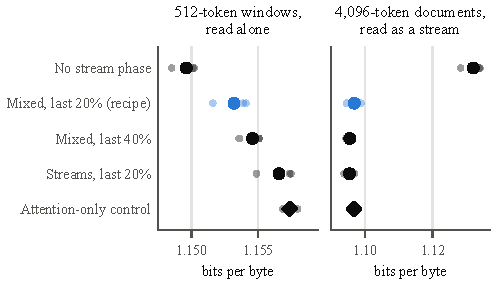
\includegraphics[width=0.5\linewidth]{figs/fig_recipes.pdf}
\caption{Stream-phase variants at 0.1B, bits per byte on 512-token windows read alone (left) and on 4,096-token documents read as a stream (right). Large markers are means of 3 seeds, and small dots are single seeds. The mixed stream phase over the last 20\% (blue) keeps most of the long-document gain at half the cost on windows alone. Averaged weights (1.2085 and 1.1523) are off the chart.}
\label{fig:recipes}
\end{figure}

\begin{table}[h]
\centering\small
\caption{BM25 search over library v2's 36.8M human passages and v1, on one H100, with v1's held-out questions as queries (\texttt{docs/library.md}). ``Same top'' is the share of queries whose top passage matches the full index's. The merged GPU index answers in 2.0 ms at the median and 2.8 ms at the 95th percentile.}
\label{tab:search}
\begin{tabular}{@{}l r r r@{}}
\toprule
Search & Index size & Median time & Same top \\
\midrule
CPU, full index & 76 GB & 426 ms & 1.00 \\
CPU, compact index (common tokens dropped, 8-bit weights) & 24.6 GB & 349 ms & 1.00 \\
GPU, compact index, part by part & 24.6 GB & 3.9 ms & 1.00 \\
GPU, each token's 100,000 best passages, merged into one index & 25.0 GB & \textbf{2.0 ms} & 0.86 \\
\bottomrule
\end{tabular}
\end{table}

\begin{table}[h]
\centering\small
\caption{Zero-shot accuracy at 0.5B, mean of 2 seeds, normalized where the task has a normalized score (\sect{20}). Means are of unrounded scores. All three models are near chance on ARC-Challenge and WinoGrande.}
\label{tab:bench}
\setlength{\tabcolsep}{3pt}
\begin{tabular}{@{}l ccc@{}}
\toprule
Task & ExeaLM & Qwen3.5-style & Llama \\
\midrule
HellaSwag \citep{zellers2019hellaswag} & \textbf{0.309} & 0.304 & 0.298 \\
ARC-Easy \citep{clark2018arc} & 0.402 & \textbf{0.408} & 0.393 \\
ARC-Challenge \citep{clark2018arc} & \textbf{0.236} & 0.234 & 0.233 \\
PIQA \citep{bisk2020piqa} & 0.584 & \textbf{0.591} & 0.584 \\
WinoGrande \citep{sakaguchi2020winogrande} & 0.495 & 0.493 & \textbf{0.508} \\
SciQ \citep{welbl2017sciq} & \textbf{0.699} & 0.667 & 0.647 \\
LAMBADA \citep{paperno2016lambada} & \textbf{0.274} & 0.254 & 0.255 \\
\midrule
Mean of 7 & \textbf{0.429} & 0.421 & 0.417 \\
\bottomrule
\end{tabular}
\end{table}

\end{document}
